%!TeX root = main.tex

\section{Esempi ed osservazioni utili}

\begin{esempio}[A cosa serve uno spazio normato e il prodotto scalare?]
	Prendo un SR e fisso una $(O, e_1, e_2..., e_n)$ a questo punto un vettore diventa  $$v = (x,y) = x e_1 + y e_2$$ con 
	\[
	x : \mathbb{R}^2 \rightarrow \mathbb{R} \quad \quad \quad x(v) = x = (e_1 , v)\]\[
	y : \mathbb{R}^2 \rightarrow \mathbb{R} \quad \quad \quad y(v) = y = (e_2 , v)
	\]
	$x$ e $y$ dipendono quindi dalla base. La norma di un vettore invece non dipende dalla base. Il prodotto scalare invece mi serve per distinguere due vettori della stessa norma.
\end{esempio}

\begin{esempio}[Norma su $\mathcal{D}(\mathbb{R})$]
	Si prenda $\mathcal{D}(\mathbb{R})$ lo spazio delle funzioni reali $C^\infty$ a supporto compatto. Posso definirci sopra la norma $||\cdot||_p$ si può fare perchè è liscia e avendo supporto compatto è limitata.
\end{esempio}

\subsection{Spazi di Hilbert}

\begin{esempio}[Spazi non separabili]
	\begin{itemize}
		\item \textbf{Oscilloscopio} \newline
		Vorrei ricostruire $\psi(x) = \sum c_n e^{i \omega_n x}$. Il problema però è che quando si vuole ricostruire un suono per esempio si fa uno spettro continuo in frequenze (oppure non sono dei seni multipli). Non ho infatti periodicità e quindi nessuna  serie di Fourier .
		\item \textbf{Funzioni quasi-periodiche} \newline
		Prendiamo $f,g \in C^\infty(\mathbb{R})$
		\[
		(f,g) = \lim_{R \rightarrow \infty} \frac{1}{2R} \int_{-R}^{R} dx \overline{g(x)}f(x)
		\]
		questo permette di costruire uno spazio di Hilbert $B_2(\mathbb{R})$  con la $|| \cdot ||_2$. Una base è $\{e^{i\lambda x}\}_{\lambda \in \mathbb{R}}$. Questo spazio di Hilbert non è separabile.
	\end{itemize}
\end{esempio}

\begin{esempio}[Insiemi densi]
	E' possibile lavorare con un certo insieme di funzioni e ottenere risultati che valgono per tutte le altre? Questo ci porta al concetto di insieme denso.\newline
	$\mathcal{D}(\mathbb{R})$ e $\mathcal{S}(\mathbb{R})$ sono denso in $L^2(\mathbb{R})$. Non ha senso lavorarci in dimensione finita.
\end{esempio}

\begin{esempio}[Perchè usiamo $L^2$]
	Perchè non vogliamo imporre limiti geometrici a priori sul modello.
\end{esempio}

\subsection{Spazio di Successioni}
\begin{itemize}
	\item $l^p = \{(x_n)_{n \in \mathbb{N}} \subset \mathbb{K} \mid \sum_{n=1}^\infty |x_n|^p < \infty\}$, $1 \le p < \infty$
	\item $l^\infty = \{(x_n) \subset \mathbb{K} \mid (x_n) \text{ è limitata}\}$
	\\ $(x_n) \in l^\infty \Leftrightarrow \exists C > 0 \text{ t.c. } \sup_{n \in \mathbb{N}} |x_n| \le C < \infty$
	\item $c = \{(x_n) \subset \mathbb{K} \mid (x_n) \text{ ammette limite } < \infty\}$
	\item $c_0 = \{(x_n) \subset \mathbb{K} \mid \lim_{n \to \infty} x_n = 0\}$
	\item $c_{00} = \{(x_n) \subset \mathbb{K} \mid x_n \text{ defi nitivamente nulla}\}$
\end{itemize}

\paragraph{Norme}
\begin{itemize}
	\item Su $l^p$: $||x||_p = \left(\sum_{n=1}^\infty |x_n|^p\right)^{1/p}$
	\item Su $l^\infty, c, c_0, c_{00}$: $||x||_\infty := \sup_{n \in \mathbb{N}} |x_n|$
\end{itemize}

\subsubsection*{Inclusioni Naturali tra Spazi $l^p / c / c_0 / c_{00}$}
Per $1 \le p < r < \infty$:
\[ c_{00} \subset l^p \subset l^r \subset c_0 \subset c \subset l^\infty \]
$c_{00}$ è denso in $l^p$ (per $p<\infty$) e in $c_0$. Le inclusioni sono continue.
\begin{itemize}
	\item $(l^p, ||\cdot||_p)$ è Banach.
	\item $(l^2, ||\cdot||_2)$ con $(x,y) = \sum_{n=1}^\infty \overline{x_n} y_n$ è Hilbert.
	\item $(c_0, ||\cdot||_\infty)$ e $(c, ||\cdot||_\infty)$ sono Banach (sono sottospazi chiusi di $l^\infty$).
	\item $(c_{00}, ||\cdot||_\infty)$ NON è banach (perchè non è completo).\newline
	Controesempio: Si consideri la successione $(x^k)_{k \in \mathbb{N}}$ in $c_{00}$ data da $x_n^k = \begin{cases} 1/n & \text{se } 1 \le n \le k \\ 0 & \text{altrimenti} \end{cases}$.
	\begin{itemize}
		\item È una successione di Cauchy in $l^\infty$: per $l \ge 1$,
		\[ ||x^k - x^{k+l}||_\infty = \sup_{n=k+1}^{k+l} \left|\frac{1}{n}\right| = \frac{1}{k+1} \xrightarrow[k \to \infty]{} 0 \]
		\item Ma $(x^k)$ converge in $l^\infty$ alla successione $x = (1/n)_{n \in \mathbb{N}}$.
		\item $x \in c_0$ (perché $1/n \to 0$), ma $x \notin c_{00}$ (non è definitivamente nulla).
		\item Quindi $c_{00}$ non è uno spazio chiuso in $c_0$, perciò non è completo.
	\end{itemize}
\end{itemize}

\subsubsection*{Disuguaglianza di Hölder}
$\forall x \in l^p, \forall y \in l^q$ t.c. $\frac{1}{p} + \frac{1}{q} = 1$:
\[ \sum_{n=1}^\infty |x_n y_n| \le ||x||_p ||y||_q \]
Se $p=q=2 \implies$ Disuguaglianza di Cauchy-Schwartz.

\subsubsection*{Separabilità di $l^p$}
\begin{itemize}
	\item $l^p$ è separabile per $1 \le p < \infty$. ($l^\infty$ non è separabile).
	\item Uno spazio è separabile $\Leftrightarrow \exists$ un sottospazio denso numerabile.
	\item $c_{00}$ (in particolare l'insieme delle successioni a valori razionali) è denso in $(l^p, ||\cdot||_p)$ per $1 \le p < \infty$.
	\item $\overline{c_{00}}^{||\cdot||_p} = l^p$.
	\item $(\forall x \in l^p, \exists (x^k) \subset c_{00} \text{ t.c. } ||x^k - x||_p \to 0)$
\end{itemize}

\subsubsection*{Riflessività}
Def: Uno spazio normato $(X, ||\cdot||_X)$ è riflessivo se l'immersione canonica $J: X \to X^{\star\star}$ è suriettiva.
\begin{itemize}
	\item $J: x \mapsto \delta_x$
	\item $\delta_x: X^\star \to \mathbb{K}$ è un funzionale lineare e continuo (un elemento del biduale $X^{\star\star}$) definito da:
	\[ f \mapsto \delta_x(f) = f(x) \]
	\item $X^\star = \{f: X \to \mathbb{K}, \text{lineare e continuo}\}$ (duale topologico)
	\item $X^{\star\star} = (X^\star)^\star$ (biduale topologico)
\end{itemize}
\begin{itemize}
	\item La riflessività vale per $(l^p, ||\cdot||_p)$ con $1 < p < \infty$.
	\item Tutti gli spazi di Hilbert sono riflessivi.
\end{itemize}


\subsection{Spazi di Funzioni $L^p(\mathbb{R}^n)$ ($p \in [1, +\infty]$)}
Sia $\Omega \subseteq \mathbb{R}^n$ un aperto e $\mu$ la misura di Lebesgue.

\begin{itemize}
	\item $L^p(\Omega) = \{ [f]: \Omega \to \mathbb{K} \mid \int_\Omega |f(x)|^p d^n x < \infty \}$, per $1 \le p < \infty$.
	\item $L^\infty(\Omega) = \{ [f]: \Omega \to \mathbb{K} \mid \exists C > 0 \text{ t.c. } |f(x)| \le C \text{ q.o. in } \Omega \}$
	\item La norma in $L^\infty$ è $||f||_{L^\infty} = \inf \{ C > 0 \mid |f(x)| \le C \text{ q.o. in } \Omega \}$ (estremo superiore essenziale).
\end{itemize}
Si considerano classi di equivalenza $[f]$ (funzioni uguali quasi ovunque) affinché $||f||_{L^p} = 0 \Leftrightarrow f = 0$ q.o.

\subsubsection*{Disuguaglianza di Hölder per $L^p$}
Siano $f \in L^p(\Omega)$ e $g \in L^q(\Omega)$ con $\frac{1}{p} + \frac{1}{q} = 1$.
Allora $fg \in L^1(\Omega)$ e
\[ \int_\Omega |f(x) g(x)| d^n x \le \left( \int_\Omega |f(x)|^p d^n x \right)^{1/p} \left( \int_\Omega |g(x)|^q d^n x \right)^{1/q} \]
ovvero $||fg||_{L^1} \le ||f||_{L^p} ||g||_{L^q}$.

\subsubsection*{Inclusioni Naturali}
Se $mis(\Omega) = \int_\Omega 1 d^n x < \infty$ (misura finita) e $1 \le p < r \le \infty$:
\[ L^r(\Omega) \subset L^p(\Omega) \]
L'inclusione è continua.

\subsubsection*{Riflessività}
\begin{itemize}
	\item $L^p(\Omega)$ è riflessivo per $1 < p < \infty$.
	\item $L^1(\Omega)$ e $L^\infty(\Omega)$ non sono riflessivi (in generale).
\end{itemize}

\subsubsection*{Separabilità}
\begin{itemize}
	\item $L^p(\Omega)$ è separabile per $1 \le p < \infty$.
	\item $L^\infty(\Omega)$ non è separabile (in generale).
	\item $C_0^\infty(\Omega)$ (funzioni $C^\infty$ a supporto compatto in $\Omega$) è denso in $L^p(\Omega)$ per $p < \infty$.
	\item $\overline{C_0^\infty(\Omega)}^{||\cdot||_{L^p}} = L^p(\Omega)$.
\end{itemize}

\subsubsection*{Convergenza Debole e Forte in $X^\star$}
Sia $(X, ||\cdot||_X)$ uno spazio normato e $\{f_n\} \subset X^\star$.
\begin{itemize}
	\item \textbf{Convergenza Debole (puntuale):} $f_n \rightharpoonup f$ se $f_n(x) \to f(x)$ $\forall x \in X$.
	\item \textbf{Convergenza Forte (in norma):} $f_n \to f$ se $||f_n - f||_{X^\star} \to 0$.
	\item forte $\implies$ debole.
	\item debole $\implies$ forte se $\dim X < \infty$.
\end{itemize}


\subsection{Spazi $L_{loc}^p(\mathbb{R}^n)$}
Def: $f \in L_{loc}^p(\mathbb{R}^n)$ (spazio delle funzioni localmente $p$-integrabili), $1 \le p \le \infty$, se:
\[ \forall K \subset \mathbb{R}^n \text{ compatto, } f \in L^p(K) \]
(cioè $\int_K |f(x)|^p dx < \infty$).\newline\newline
Esempi:
\begin{itemize}
	\item $f(x) \equiv c \in \mathbb{R}$. Se $c \ne 0$, $f \notin L^1(\mathbb{R})$ ma $f \in L_{loc}^1(\mathbb{R})$ (e $L_{loc}^p$ per ogni $p$).
	\item $f \in C^0(\mathbb{R}^n) \implies f \in L_{loc}^p(\mathbb{R}^n)$ per ogni $p$, perché $f$ è limitata sui compatti.
	\item $f(x) = 1/x$ (con $f(0)=0$) non è in $L_{loc}^1(\mathbb{R})$. Basta prendere un compatto $K$ che contiene $0$, ad esempio $K=[-1,1]$, e si ha $\int_{-1}^1 |1/x| dx = \infty$.
\end{itemize}
Valgono le seguenti inclusioni:
$$L^p(\R^n),C^\infty(\R^n) \subset L^1_{\text{Loc}}(\R^n) \subset  \mathcal{D}'(\R^n)$$

\subsubsection*{Lemma (Fondamentale Calcolo Variazioni, caso 1D)}
Sia $I = (a,b) \subset \mathbb{R}$, $a < b$, $f \in L_{loc}^1((a,b))$.
Se vale:
\[ \int_a^b f(x) \frac{d\varphi}{dx}(x) dx = 0 \quad \forall \varphi \in C_0^\infty((a,b)) \]
allora $\exists c \in \mathbb{R}$ t.c. $f(x) = c$ per q.o. $x \in (a,b)$.


\subsection{Richiami di Complementi di Analisi III}
Sia $\Omega \subseteq \mathbb{R}^n$ aperto.

\begin{teorema}[Teorema di Beppo Levi (Convergenza Monotona)]
	\noindent Sia $(f_n)_{n \in \mathbb{N}} \subset L^1(\Omega)$ una successione di funzioni tale che:
	\begin{itemize}
		\item $f_n \ge 0$ q.o.
		\item $f_n(x) \le f_{n+1}(x)$ q.o. $\forall n \in \mathbb{N}$ (monotona non decrescente).
	\end{itemize}
	Sia $f(x) = \lim_{n \to \infty} f_n(x)$ q.o. (il limite esiste, eventualmente $+\infty$).
	Allora:
	\[ \int_\Omega f(x) dx = \lim_{n \to \infty} \int_\Omega f_n(x) dx \]
\end{teorema}

\begin{teorema}[Lemma di Fatou]
	\noindent Sia $(f_n)_{n \in \mathbb{N}} \subset L^1(\Omega)$ una successione di funzioni tale che $f_n \ge 0$ q.o.
	Allora:
	\[ \int_\Omega \liminf_{n \to \infty} f_n(x) dx \le \liminf_{n \to \infty} \int_\Omega f_n(x) dx \]
\end{teorema}

\begin{teorema}[Teorema di Lebesgue (Convergenza Dominata)]
	\noindent Sia $(f_n)_{n \in \mathbb{N}} \subset L^1(\Omega)$ una successione di funzioni tale che:
	\begin{itemize}
		\item $f_n(x) \to f(x)$ q.o. in $\Omega$.
		\item $\exists g \in L^1(\Omega)$ (una funzione dominante) t.c. $\forall n \in \mathbb{N}$, $|f_n(x)| \le g(x)$ q.o.
	\end{itemize}
	Allora $f \in L^1(\Omega)$ e $||f_n - f||_{L^1} \to 0$ (cioè $f_n \to f$ in $L^1$).
\end{teorema}

\subsection{Spazi di Sobolev $W^{k,p}(\mathbb{R}^n)$}
Esempio (Equazione di Schrödinger per una particella libera):
\[ i \hbar \frac{\partial}{\partial t} \psi(t, \underline{x}) = -\frac{\hbar^2}{2m} \Delta \psi(t, \underline{x}) \]
Si cerca $\psi$ tale che $\psi(t, \cdot) \in L^2(\mathbb{R}^3)$ (funzione d'onda) per ogni $t$.
L'equazione contiene $\Delta \psi = \sum_i \frac{\partial^2 \psi}{\partial x_i^2}$. Per dare senso a questo operatore, non basta richiedere $\psi \in C^2$. La richiesta corretta (in termini energetici) è $\psi(t, \cdot) \in H^2(\mathbb{R}^3)$.

\subsubsection*{Definizione $W^{1,p}$ (Derivata Debole)}
Sia $\Omega \subseteq \mathbb{R}^n$ aperto, $1 \le p < \infty$.
Si dice che $u \in W^{1,p}(\Omega)$ se:
\begin{enumerate}
	\item $u \in L^p(\Omega)$
	\item $\exists f_1, \dots, f_n \in L^p(\Omega)$ tali che (integrando per parti):
	\[ \int_\Omega u \frac{\partial \varphi}{\partial x_i} dx = - \int_\Omega f_i \varphi dx \quad \forall \varphi \in C_0^\infty(\Omega), \forall i = 1, \dots, n \]
\end{enumerate}
Le funzioni $f_i$ sono uniche (q.o.) e sono chiamate \textbf{derivate deboli} di $u$. Si pone $f_i =: \frac{\partial u}{\partial x_i}$.
\begin{itemize}
	\item Se $u \in C^1(\Omega) \cap L^1(\Omega)$, le derivate deboli coincidono con le derivate classiche.
\end{itemize}

\paragraph{Norma $W^{1,p}$}
La norma standard su $W^{1,p}(\Omega)$ è:
\[ ||u||_{W^{1,p}} = \left( ||u||_{L^p}^p + ||\nabla u||_{L^p}^p \right)^{1/p} = \left( \int_\Omega |u|^p dx + \sum_{i=1}^n \int_\Omega \left|\frac{\partial u}{\partial x_i}\right|^p dx \right)^{1/p} \]
(Per $p=\infty$ si usa la somma delle norme $L^\infty$).

\paragraph{Proprietà}
$(W^{1,p}(\Omega), ||\cdot||_{W^{1,p}})$ è uno spazio di Banach.
\begin{itemize}
	\item È separabile per $1 \le p < \infty$.
	\item È riflessivo per $1 < p < \infty$.
	\item Per $p=2$: $W^{1,2}(\Omega) = H^1(\Omega)$ è uno spazio di Hilbert con prodotto scalare:
	\[ (u, v)_{H^1} := \int_\Omega (u v + \nabla u \cdot \nabla v) dx \]
\end{itemize}

\subsubsection*{Definizione $W^{k,p}$}
Sia $\Omega \subseteq \mathbb{R}^n$ aperto. Per $k \in \mathbb{N}$:
\[ W^{k,p}(\Omega) = \{ u \in L^p(\Omega) \mid D^\alpha u \in L^p(\Omega) \quad \forall |\alpha| \le k \} \]
dove $\alpha = (\alpha_1, \dots, \alpha_n) \in \mathbb{N}_0^n$ è un multi-indice, $|\alpha| = \sum \alpha_i$ è l'ordine della derivata, e $D^\alpha u = \frac{\partial^{|\alpha|} u}{\partial x_1^{\alpha_1} \dots \partial x_n^{\alpha_n}}$ è la derivata debole.
\begin{itemize}
	\item $W^{k,2}(\Omega) =: H^k(\Omega)$ (Spazi di Hilbert)
	\item $W^{0,p}(\Omega) = L^p(\Omega)$, quindi $H^0 = L^2$.
	\item Esempio Schrödinger: $\psi(t, \cdot) \in H^2(\mathbb{R}^3) = \{ \psi \in L^2(\mathbb{R}^3) \mid \partial_i \psi \in L^2, \partial_i \partial_j \psi \in L^2 \}$.
\end{itemize}

\subsubsection*{Teoremi di Embedding di Sobolev}
I teoremi di Sobolev (o immersioni) stabiliscono relazioni tra gli spazi $W^{k,p}$ e gli spazi $C^m$ (spazi di funzioni continue con $m$ derivate continue).
\newline
Se $k - n/p > m$ (dove $m$ è un intero $\ge 0$), allora $W^{k,p}(\mathbb{R}^n) \subset C^m(\mathbb{R}^n)$.\newline
Una formula sintetica è: $u \in W^{k,p}(\mathbb{R}^n) \implies u \in C^m(\mathbb{R}^n)$ con $m = \lfloor k - n/p \rfloor$.
\newline
\begin{osservazione}[]
	\begin{itemize}
		\item $u \in H^2(\mathbb{R}^3)$. Qui $k=2, p=2, n=3$.
		\item $m = \lfloor 2 - 3/2 \rfloor = \lfloor 0.5 \rfloor = 0$.
		\item Quindi $H^2(\mathbb{R}^3) \subset C^0(\mathbb{R}^3)$.
		\item Questo significa che una funzione $H^2$ (dopo eventuale modifica su un insieme di misura nulla) è continua e limitata.
		\item Questo è fondamentale per poter "valutare la funzione $\psi$ in un punto $x_0$", $\psi(x_0)$, operazione che non ha senso per una generica funzione $L^2$.
	\end{itemize}
\end{osservazione}

\subsection{Operatori}
\begin{esempio}[Operatore posizione]
	Prendiamo $\mathcal{H} = L^2((0,1))$ e definiamo
	\[
	\hat{X} : L^2((0,1)) \rightarrowtail L^2((0,1))  \quad \quad \quad \quad \hat{X}\psi = x \psi
	\]
	possiamo calcolare la norma usando che 
	\[
	\int_{0}^{1} dx |x \psi(x)|^2 \leq 	\int_{0}^{1} dx |\psi(x)|^2 \Rightarrow || \hat{X} || \leq 1
	\]
	Se però $\mathcal{H} = L^2(\mathbb{R})$ allora posso prendere $\psi(x) \in  L^2(\mathbb{R})$ tale che
	\begin{equation*}
		f(x) =
		\begin{cases}
			0 &\quad x < 1 \\
			\frac{1}{x} &\quad x \geq 1
		\end{cases}
	\end{equation*}
	ma $\hat{X} \psi \notin L^2(\mathbb{R})$ quindi gli operatori non limitati hanno bisogno di una teoria più estesa. \newline
	Vogliamo costruire l'aggiunto di $\hat{X}$, supponiamo di saperne l'esistenza. Possiamo usare
	\[
	(\phi, \hat{X}\psi)=\int_0^1 dx \overline{\phi(x)}x\psi(x) = \int_0^1 dx \overline{x}\overline{\phi(x)}\psi(x)  = (\hat{X} \phi, \psi)
	\]
	quindi è autoaggiunto.\newline
	Prendiamo $\mathcal{H} = L^2((0,1))$, proviamo a trovarne gli autovalori
	\[
	\hat{X} \psi = \lambda \psi
	\]
	anche se mi aspetto a priori che $\lambda = x$ $\forall \psi \in [0,1]$ $\exists \psi \neq 0 \in W_{\lambda}$ quindi deve esistere un sottospazio ortogonale a $W_{\lambda}$ quindi ho trovato una decomposizione con cardinalità di $[0,1]$, ma questo è assurdo perchè $L^2$ è separabile. Abbiamo postulato che $\hat{X}$ sia l'operatore giusto per la posizione magari ha autovalori diversi da quelli che ci aspttiamo però $\forall x$ troviamo il $\lambda$ tale che  
	\[
	x \psi(x) = \lambda \psi(x) \iff \psi(x) = 0
	\] 
	quindi non ho autovalori. Proviamo ad estendere la definizione di autovalore. Con le matrici quadrate 1 
	\[
	T v = \lambda v \iff (T - v \mathds{1}) = 0 \Rightarrow \nexists (T - v \mathds{1})^{-1}
	\]
	quindi se esiste l'inversa allora non $\lambda$ non è un autovalore. In dimensione finita non ho fatto niente. Vediamo il caso di $\hat{X}$
	\[
	\exists (\hat{X} - \lambda \mathds{1})^{-1} \text{   t.c.   } ((\hat{X} - \lambda \mathds{1})^{-1}\psi)(x) = \frac{1}{x - \lambda} \psi(x) \Rightarrow (\hat{X} - \lambda \mathds{1})^{-1} := \frac{1}{x - \lambda}
	\]
	Se $\lambda \in \mathbb{C} \setminus \mathbb{R} \cup \mathbb{R} \setminus[0,1] $ 
	\[
	\int_0^1 dx |\frac{\psi}{x - \lambda}|^2 < \infty
	\]
	quindi ho l'inverso ben definito. Dato che l'unico intervallo in cui quell'integrale non è definito sono $[0,1]$ non ho l'inversa quindi sono autovalori. Quindi possiamo introdurre questa nuova definizione pagando il prezzo di non avere più autofunzioni in $L^2$, useremo le distribuzioni.\newline
	Questo operatore ha un ottimo comportamento nei limitati. Cambiando gli autovalori a seconda dello spazio in cui ci troviamo.
\end{esempio}

\begin{esempio}[Operatore parità]
	Prendiamo $\mathcal{H} = L^2(\mathbb{R})$ e definiamo
	\[
	\hat{P} : L^2(\mathbb{R}) \rightarrowtail L^2(\mathbb{R})  \quad \quad \quad \quad \hat{P}\psi(x) = \psi(-x)
	\]
	possiamo calcolare la norma
	\[
	|| \hat{P} || = 1
	\]
	esso è anche unitario, cioè non cambia le norme. \newline
	Troviamo gli autovalori di $P$
	\[
	P\psi = \lambda \psi \rightarrow \psi(-x) = \lambda \psi(+x)
	\]
	usando $P^2$ possiamo trovare che $\lambda ^ 2 = 1$. Definiamo $\psi_{\pm} = \frac{\psi(x) \pm \psi(-x)}{2}$  si mostra che sono autovalori di $P$. Quindi ogni funzione di $L^2$ può essere decomposta in due funzioni, la parte pari e la parte dispari. \newline
	Prendiamo una carica $q$ a destra di un semispazio infinito conduttore, prendiamo $\vec{E_q} = k \frac{q}{r^2} \hat{r}$ come se non ci fosse la parete e inoltre voglio che $\vec{E_q}(x = 0) = 0$ prendo quindi la parte dispari e rimane una soluzione delle Maxwell. Se invece avessi $\partial_x \vec{E_q} (x = 0) = 0$ prendo la parte pari. \newline
	Si può dimostrare che l'operatore che prende la parte pari (dispari) sia un proiettore.
\end{esempio}
\begin{esempio}[Operatori finito dimensionali]
	Un operatore su $\mathbb{C}^n$ è sempre rappresentabile tramite una matrice ed è sempre limitato. I seguenti sono indipendenti dalla base scelta
	\begin{itemize}
		\item Determinante (dipende dal prodotto degli autovalori)
		\item Traccia (dipende dalla somma degli autovalori)
		\item Autovalori
	\end{itemize}
	dato che voglio estrarre informazioni da un sistema fisico che è indipendente dalla base, queste devono essere contenute negli autovalori. Da ciò deriva il postulato della misura.  Ci interessiamo però di misure reali quindi vorremmo che i nostri autovalori fossero numeri reali.
	Data una $A : \mathbb{C}^n \rightarrow \mathbb{C}^n$ e una b.o.c $\{e_i\}$ allora $A_{ij} = (e_i, Ae_j)$ se A è diagonalizzabile allora esiste una $U$ tale che
	\[
	UAU^{-1} = \sum \lambda_i P_i \quad \quad \quad \tilde{P}_i := U^{-1}PU \Rightarrow A = \sum \lambda_i \tilde{P}_i
	\]
	tramite il teorema spettrale si dimostra che $A = \bar{A}^\dagger  = A^\star$
\end{esempio}
\begin{esempio}[Operatore impulso]
	Prendiamo una $\psi \in L^2$
	\begin{equation*}
		\psi(x) =
		\begin{cases}
			x^{-1/4} &\quad 0 \leq x < 1 \\
			0 &\quad altrove
		\end{cases}
	\end{equation*}
	applicando $\frac{d}{dx}$ usciamo da $L^2$. Ora provo a calcolare l'aggiunto
	\[
	\left(\phi, -i \frac{d \psi}{dx}\right) = -i \int_0^1 dx \overline{\phi(x)} \frac{d \psi}{dx} (x) = -i \overline{\phi}\psi |_0^1 + \int_0^1 dx \overline{\left(-i\frac{d \phi}{dx}\right)} \psi
	\]
	questo termine di bordo va rimosso. \newline
	Questo operatore ha un ottimo comportamento negli illimitati, sistema il comportamento degli stati all'infinito e peggiora le singolarità in zero. Cambiando gli autovalori a seconda dello spazio in cui ci troviamo. Se lo spazio è limitato P e T NON sono più autoaggiunti. \newline
	Prendiamo quindi $\mathcal{H} = L^2 (0,\infty)$, che è assimilabile al caso di una particella contro una parete e supponiamo inizialmente di prendere 
	\[
	\hat{P} = -i \frac{d}{dx} \quad \quad \quad D(\hat{P}) = C^\infty_0(0, \infty)
	\]
	stando attenti a prendere l'intervallo aperto e non chiuso se no si ammettono funzioni che non si annullano in 0. Quindi si trova che
	\[
	\left(\phi, -i \frac{d \psi}{dx}\right) = -i \int_0^1 dx \overline{\phi(x)} \frac{d \psi}{dx} (x) = -i \overline{\phi}\psi |_0^1 + \int_0^1 dx \overline{\left(-i\frac{d \phi}{dx}\right)} \psi = 
	\left(\hat{P}^\star \phi, \psi\right)
	\]
	dove l'ultima uguaglianza ha senso se e solo se
	\begin{enumerate}
		\item il dominio di $\hat{P}$ permette l'annullamento del termine di bordo
		\item $\psi \in L^2$  e $\phi' \in L^2$ $\Rightarrow$ $\psi \phi' \in L^1$ 
	\end{enumerate}
	quindi troviamo che $D(\hat{P}^\star)$ è massimale, cioè tutte le funzioni tali che la loro derivata è in $L^2$. A questo punto usiamo la teoria degli indici di difetto di Von Neumann, trovando il $ker(P^\star \pm i \Identity)$, risolvendo le due equazioni differenziali si arriva a scartare la soluzione esponenziale crescente perchè non è in $L^2(0, \infty)$ ma a tenere l'altra. Questo fa si che le dimensioni degli spazi siano diverse e quindi P non è autoaggiunto e quindi neanche un'osservabile fisica di quel sistema. Capiamo cosa significa, mettiamo caso di avere l'hamiltoniana di particella libera 
	\[
	\hat{H} = \hat{T} \quad \quad \hat{T} = -\frac{\hbar^2}{2m} \frac{d^2}{dx^2}
	\]
	(da notare che non ho fatto comparire P), che applicata alla soluzione esponenziale negativa mi restituisce un'autovalore negativo. Questo autovalore non è rimuovibile come in fisica classica aggiungendo una costante in quanto in MQ questo non è più valido. P non può più essere autoaggiunto, in quanto se questo fosse vero, avrei che
	\[
	\hat{P} = \sqrt{(2m \hat{H})}
	\]
	e quindi avrebbe un autovalore complesso, il che non lo renderebbe autoaggiunto (fisico).
	A livello sperimentale quello che si fa è misurare sempre l'energia e mai l'impulso. Misurando vicino alla parete ci si accorge di questa soluzione e di questo autovalore, mentre mettendoci molto lontano dalle pareti questo effetto non viene distinto dal detector e si può lavorare con l'ipotesi di $\Hspace = L^2(\R)$.
	\newline
	Nel caso $\Hspace = L^2(0,1)$ si trova che $d_+ = d_- = 1$ e quindi P risulta essere un buon osservabile. Quindi ho una mappa $U : \C \rightarrow \C$  tra i due sottospazi $\mathcal{N}_\pm$ che manda $z \mapsto e^{i \alpha} z$ rappresentando un'isometria tra i due spazi. Costruendo tramite essa le estensioni autoaggiunte, si può notare che la scelta di $\alpha$ rappresenta la scelta della condizione al contorno del problema.
\end{esempio}
\begin{esempio}[Operatori compatti]
	Possiamo immaginarceli come matrici infinite. Vorrei fare il conto di $\langle A \rangle$ con un certo $\psi = (\alpha, \beta)$ senza utilizzare una base. Non è che forse $\langle A \rangle = Tr(\rho A)$ dove 
	\[
	\rho = \begin{pmatrix}
		|\alpha|^2& \bar{\alpha} \beta \\
		\bar{\beta} \alpha & |\beta|^2 
	\end{pmatrix}
	\]
	facendo il conto si trova che è vero. In MQ si può generalizzare uno stato con queste matrici di densità. In spazi infinito-dimensionali abbiamo bisogno di oggetti del genere con traccia finita, quali sono? Operatori classe traccia che sono compatti.\newline
	Gli operatori compatti garantiscono che:
	\begin{enumerate}
		\item Gli autovalori ordinati tendono a 0
		\item Ogni autovalore ha molteplicità finita
	\end{enumerate}
	quindi abbiamo speranza che la traccia converga.
\end{esempio}

\begin{esempio}[Operatori non limitati]
	Un esempio generale di operatore non limitato è (con $\Hspace= L^2(\R)$) 
	\[
	T = \sum_{k=0}^N c_k(x) \frac{d^k}{dx^k}
	\]
	se ho $\psi \in \mathcal{D}(\R)$ $T\psi \in \mathcal{D}(\R)$ e sono tutti stati.
\end{esempio}

\begin{esempio}[Operatori densi]
	Definiamo
	\[
	\hat{T} = -i \frac{d}{dx} \quad \quad \quad \hat{K} = - \frac{d^2}{dx^2}
	\]
	il dominio massimale è quello per cui ha senso applicarci l'impulso.
	\[
	D_{\text{massimale}}(\hat{T}) = H^1(\R)  \quad \quad \quad D_{\text{massimale}}(\hat{K}) = H^2(\R)
	\]
	dobbiamo anche assicurarci che (la corrente conservata)
	\[
	\lim_{x \rightarrow \infty} \overline{\psi} \frac{d \psi}{dx} = 0
	\]
	questa va a 0 solo in una dimensione su $H^1$  ma non in $\R^3$, questa va a 0 ma per tanti altri matti motivi.\newline
	Un caso sensato in cui possiamo fare i conti senza soffrire è $\mathcal{D}(\R) = D_0(\hat{T})$ che è denso in tanti spazi e va tutto bene. Proviamo a trovare l'aggiunto
	\[
	(\phi, T\psi) = -i\int_\R \overline{\phi(x)} \frac{d \psi}{dx} = -i \overline{\phi} \psi \bigg|_{-\infty} ^{+\infty} + i\int_\R \frac{d \overline{\phi}(x)}{dx} \psi(x)
	\]
	dove il termine di bordo muore senza problemi, se avessi usato $H^1$ andava bene in una dimensione ma in tre assolutamente no. Continua però a non essere definito bene il secondo integrale, potrebbe essere comunque un integrale divergente. Se ho però la derivata di $\phi \in L^2(\R)$ allora va bene perchè il prodotto di due $L^2$ mi da una $L^1$ e quell'integrale si fa. Allora a quel punto posso dire che quel conto fa $(\hat{T} ^\star \phi, \psi)$ ottengo quindi che
	\[
	D(\hat{T}) = \mathcal{D}(\R) \quad \quad \quad \quad D(\hat{T}^\star) = H^1(\R)
	\]
	però
	\[
	T^\star \psi = -i \frac{d \psi}{dx} \quad \Rightarrow \quad T \subset T^\star
	\]
	La domanda che mi faccio è, esiste un S tale che
	\[
	T \subset S \subset T^\star \quad \text{t.c.} \quad S = S^\star
	\]
	La risposta può essere, non si può fare (operatore P su una semiretta), si può fare ed è unico (operatore P su $\R$), ci sono infiniti modi di farlo. 
\end{esempio}

\subsection{Varie su operatori}
\begin{esempio}[Aggiunto di A]
	Scelgo $A \in \mathcal{B}(\mathcal{H})$ e suppongo che $A \psi = \lambda_1 \psi$ quindi il sistema non cambia e io posso confrontarlo con uno stato di controllo $(\psi, \lambda_1 \psi) = (\psi, A \psi) = \lambda_1$ (dato che $|| \psi || = 1$). In generale posso farlo con un qualunque vettore di comtrollo o un array di essi. Posso ricavare la stessa informazione agendo sullo stato di controllo invece che sul sistema fisico? In altre parole, esiste un certo B tale che $(\phi, A \psi) = (B\phi, psi)$? La risposta ci porta all'aggiunto di A. Se questo operatore è lo stesso A si dice che è autoaggiunto e ha autovalori reali.
\end{esempio}


\begin{esempio}[Modulo di un operatore]
	Prendiamo un $A \in \mathcal{B}(\mathbb{C}^n)$ diagonalizzabile e prendiamo una funzione $f : \mathbb{C} \rightarrow \mathbb{C}
	$\[
	A = \sum \lambda_i P_{\lambda_i}  \Rightarrow f(A) := \sum f(\lambda_i )P_{\lambda_i}
	\]
	il modulo serve perchè vorrei decomporre una matrice come decompongo un numero complesso in fase e modulo. A questo punto $f$ la scelgo come la funzione radice.
\end{esempio}

\begin{esempio}[Traccia di un operatore]
	Prendiamo per semplicità una matrice, la traccia di A posso definirla anche nel caso infinito dimensionale, ma converge? Ipotizziamo che la traccia sia la somma infinita dei suoi autovalori
	\[
	TrA = \sum^\infty_{j=1} \lambda_j
	\]
	Per il teorema di Riemann-Dini, dato un numero reale e una serie semplicemente convergente ma non assolutamente convergente (come $\sum^\infty \frac{(-1)^{n+1}}{n} = ln2$), esiste una permutazione di termini di tale successione che ha converge a quel numero. Questo è un problema in MQ perchè potrei avere stati normalizzati a seconda della permutazione della serie. Quindi va richiesta la convergenza assoluta. Facciamo un esempio in cui le cose vanno male.\newline Prendimamo un operatore $T : \mathcal{H} \in \mathcal{H}$ e un vettore che scomponiamo sulla base standard ${e_n}$
	\[
	\psi = \sum^\infty c_n e_n \quad \quad \Rightarrow \quad \quad T\psi := \sum^\infty \frac{(-1)^{n+1}}{n} c_n e_n
	\]
	T si può mostrare che è limitato quindi $T \in \mathcal{B}(\mathcal{H})$ e che $|| T || \leq 1$. Però
	\[
	Tr T = \sum^\infty \frac{(-1)^{n+1}}{n} = ln2
	\]
	Ora se cambio base, e quindi scelgo i vettori della nuova base prendendone due dispari e uno pari... cioè $v_1 = e_1$ $v_2 = e_3$ $v_3 = e_2$ $v_4 = e_5$... ottengo che
	\[
	TrT = \sum^\infty \left[\frac{1}{4k-3} +  \frac{1}{4k-1} -  \frac{1}{2k} \right]= \frac{3}{2} ln2
	\]
	infatti non è classe traccia e non può essere uno stato quantistico.
\end{esempio}

\begin{esempio}[Chiusura di un operatore]
	Negli spazi finito dimensionali è come la continuità però non vediamola così. \newline
	Un operatore non chiuso è uno nel dominio non ci sono alcuni punti, come una retta che non ha il punto in zero. Uno che è chiudibile è uno che posso dire il suo valore dove non è definito.
\end{esempio}

% - 
\begin{teorema}[Completezza degli operatori limitati]
	Siano $X$ uno spazio normato e $Y$ uno spazio di Banach. Allora lo spazio degli operatori lineari limitati $\mathcal{B}(X,Y)$ è uno spazio di Banach (cioè completo rispetto alla norma operatoriale).
	$$ \|T\|_{\mathcal{B}(X,Y)} = \sup_{x \in X \setminus \{0\}} \frac{\|Tx\|_Y}{\|x\|_X} $$
	In questo caso specifico, $X=Y=\Hspace$ è Hilbert $\implies \mathcal{B}(\Hspace)$ è Banach.
\end{teorema}

% - 
\begin{teorema}[Norma operatoriale e Spazi di Banach]
	Se $X, Y$ sono spazi normati, $\mathcal{B}(X,Y)$ è normato con norma $\|T\| = \sup_{x \neq 0} \frac{\|Tx\|}{\|x\|}$. Se $Y$ è Banach, allora $\mathcal{B}(X,Y)$ è Banach.
	\emph{Dimostrazione (cenni):} Se $(T_n)_n$ è Cauchy in $\mathcal{B}(X,Y)$, allora per ogni $x$, $(T_n x)_n$ è Cauchy in $Y$. Poiché $Y$ è completo, $T_n x \to y$. Si definisce $Tx := y$. Si dimostra poi che $T$ è limitato e $T_n \to T$ in norma.
\end{teorema}




\begin{esempio}[Equivalenza Unitaria]
	Siano $T: D(T) \to \Hspace$ e $T': D(T') \to \Hspace'$ con $D(T') = U D(T)$ e $T' = UTU^{-1}$, dove $U: \Hspace \to \Hspace'$ è unitario.
	Provare le seguenti proprietà:
	\begin{itemize}
		\item[(1)] \textbf{T chiudibile $\implies$ T' chiudibile.}
		Definiamo $\overline{T'} = U \overline{T} U^{-1}$. Poiché $\overline{T}$ è chiuso, si verifica che questa è la chiusura di $T'$.
		$$ \overline{T'}|_{D(T')} = U \overline{T}|_{D(T)} U^{-1} = U T U^{-1} = T' $$
		
		\item[(2)] \textbf{T chiuso $\iff$ T' chiuso.}
		Ricordiamo che $T$ è chiuso se il grafico $\Gamma(T)$ è chiuso.
		Sia $\xi_n = U x_n \in D(T')$. Se $\xi_n \to \xi$ e $T' \xi_n \to \eta$, dobbiamo mostrare che $\xi \in D(T')$ e $T'\xi = \eta$.
		Dato che $U$ è unitario (quindi isometrico e invertibile), la convergenza di $\xi_n$ implica la convergenza di $x_n$. Essendo $T$ chiuso, le relazioni si trasportano tramite $U$.
		$$ T'\xi_n = U T U^{-1} (U x_n) = U T x_n \to U T x = T' \xi $$
		
		\item[(3)] \textbf{T hermitiano $\implies$ T' hermitiano.}
		$T$ hermitiano: $\innerprod{y}{Tx} = \innerprod{Ty}{x}$.
		Siano $x', y' \in D(T')$. Esistono $x, y \in D(T)$ tali che $x' = Ux, y' = Uy$.
		$$ \innerprod{y'}{T'x'}_{\Hspace'} = \innerprod{Uy}{UTU^{-1}Ux}_{\Hspace'} = \innerprod{Uy}{UTx}_{\Hspace'} = \innerprod{y}{Tx}_{\Hspace} $$
		$$ = \innerprod{Ty}{x}_{\Hspace} = \innerprod{UTy}{Ux}_{\Hspace'} = \innerprod{T'y'}{x'}_{\Hspace'} $$
		
		\item[(4)] \textbf{T simmetrico $\implies$ T' simmetrico.}
		Simmetrico significa Hermitiano + $D(T)$ denso.
		Abbiamo già provato l'hermiticità. La densità di $D(T')$ segue dalla densità di $D(T)$ e dalla suriettività/continuità di $U$. Se $\varphi_n \to \varphi$ in $\Hspace$, allora $U\varphi_n \to U\varphi$ in $\Hspace'$.
		
		\item[(5)] \textbf{T normale $\iff$ T' normale.}
		Normale significa $TT^* = T^*T$.
		Calcoliamo l'aggiunto: $(T')^* = (UTU^{-1})^* = (U^{-1})^* T^* U^* = U T^* U^{-1}$.
		$$ T'(T')^* = (UTU^{-1})(UT^*U^{-1}) = U T T^* U^{-1} $$
		Se $T$ è normale, $U T T^* U^{-1} = U T^* T U^{-1} = (T')^* T'$.
	\end{itemize}
\end{esempio}

\subsection{Distribuzioni}
\begin{esempio}[Distribuzioni tramite funzioni $L^1_{\text{Loc}}$]
	Sia $\psi \in L^1(\R)$ allora il funzionale $u_\psi : \D \in \C$ tale che
	\[
	f \mapsto u_{\psi}(f) := \int_\R dx f(x) \psi(x)
	\]
	(che esiste sicuramente) è una distribuzione?  Cioè è continuo?\newline Si verifica facilmente che è sequenzialmente continua. 
	\[
	\bigg|\int_\R dx f_j(x) \psi(x)\bigg| \leq \int_\R dx |f_j(x)| |\psi| \leq M\int_\R dx |\psi| = M'
	\]
	dove l'ultima disuguaglianza è data perchè è a supporto compatto con M massimo. Per convergenza dominata posso passare il limite sotto al segno d'integrale e ottengo che tutto tende a 0. Quindi è sequenzialmente continua quindi possiamo scrivere impropriamente che 
	\[
	L^1_{\text{Loc}} \subset \Dp 
	\]
	che sono le funzioni integrabili su tutti i compatti di $\R$. Inoltre si ha che
	\[
	L^p(\R) \subset L^1_{\text{Loc}} \quad \quad \quad \forall p \in \N
	\]
	quindi la MQ sta denrto $\Dp$ se consideriamo $p=2$.
\end{esempio}

\begin{esempio}[Derivata di funzioni non derivabili]
	La theta di Heaviside è $L^1_{\text{Loc}}(\R)$ ed è il prototipo di situazioni fisiche nelle quali ho un campo tangente a una superfice che dentro di essa deve essere nullo (conduttore, lago, tubo...). La componente tangente salta da un certo numero a 0. Come deriviamo una funzione del genere?
	\[
	\frac{\Theta(x)}{dx}(f) = -\Theta \left(\frac{df}{dx}\right) = -\int_\R dx \Theta(x)\frac{df}{dx} =  -\int_0^\infty dx \frac{df}{dx} = -f(x)|_0^\infty = f(0) = \delta(f)
	\]
	Ora posso derivare qualunque cosa. Per esempio $f(x) = |x|$, derivata otteniamo 
	\[
	\text{sign}(x) = \Theta(x) - \Theta(-x)
	\]
	e quindi
	\[
	\frac{d}{dx} \text{sign}(x)= \frac{d}{dx}\Theta(x) -\frac{d}{dx}\Theta(-x) = 2 \delta
	\]
	Fondamentalemente quando derivo qualcosa non derivabile (con derivabilità di salto), in ogni punto di salto ottengo una delta.
\end{esempio}

\begin{esempio}[Posso integrare su $\Dp$?]
	Se voglio mantenere la linearità (e quindi l'invarianza per traslazioni) no. Se no si fa e si chiama path integral.
\end{esempio}

\begin{esempio}[Serie di Taylor]
	Prendiamo la serie di Taylor centrata in 0 di una f
	\[
	f(x) = \sum_{n=0}^\infty \frac{f^{(n)}(x)}{n!}x^n = \left[\sum_{n=0}^\infty \frac{(-1)^n}{n!}x^n \delta^{(n)} \right](f)
	\]
	si nota che
	\[
	x \delta^{(1)}(f) = \delta^{(1)}(xf) = -\delta(f + xf')  = -\delta(f) - 0 \delta(f')= -\delta(f)
	\]
\end{esempio}

\subsection{Osservazioni sulla MQ}
\begin{esempio}[Misure in MQ]
	In MQ ho una corrispondenza biunivoca tra osservabili e operatori su $L^2(\mathbb{R})$
	\[
	A : L^2(\mathbb{R}) \rightarrow L^2(\mathbb{R})
	\]
	voglio che il processo di misura restituisca sempre qualcosa nello stesso spazio e voglio che non sia troppo diverso dallo stato iniziale (che non cambino le propietà topologiche degli insiemi input) i.e. voglio continuità degli operatori. Per esempio prendiamo $U_a$ operatore che agisce su $\mathcal{D}(\mathbb{R})$ come
	\[
	(U_af)(x) = f(x-a)
	\]
	questa cosa funziona perchè l'integrale di Lebesgue è invariante per traslazioni. \newline
	Prendo uno stato $\psi \in \mathcal{H}$ ci faccio agire $A$ (operatore su questo spazio) e ottengo un nuovo stato. Siamo interessati quale sia la "differenza" tra questo nuovo stato e quello inziale. Quindi viene introdotta la norma di un operatore.
\end{esempio}
\begin{esempio}[Successione di misure]
	Vorrei inoltre poter fare una successione di misure sul mio sistema che generano una successione di stati che non so neanche se converge. Vorrei che a partire dai dati sperimentali riuscissi a concludere che la successione converge a qualcosa che posso approssimare a meno di un $\epsilon$. Devo avere quindi uno spazio in cui $Cauchy \iff Convergente$. I limiti sono SEMPRE in norma.
\end{esempio}
\begin{esempio}[Perchè la MQ è basata su $L^2(\mathbb{R})$]
	Si consideri
	\[
	\varepsilon(E,B) = \int_\mathbb{R} dx(|E|^2 + |B|^2)
	\]
	quest'integrale ovviamente deve convergere, ma esistono soluzioni delle Maxwell che lo fanno divergere $e^{x-t}$. Quindi si richiede che $E,B \in L^2(\mathbb{R})$. Gli spazi di Hilbert separabili vogliono mantenere la finitezza di queste grandezze fisiche.
\end{esempio}

\begin{esempio}[Statistica di Bose-Einstein e oscillatore armonico quantistico]
	Si prenda l'oscillatore armonico quantistico
	\[
	\hat{H} = \frac{\hat{P}^2}{2m} + \frac{1}{2} m\omega^2 \hat{Q}^2
	\]
	esso presenta uno spettro discreto $E_n = \hbar \omega\left(n + \frac{1}{2}\right)$, da dove salta fuori l'ipotesi di Planck?
	\newline Dato $\beta = (k_B T)^{-1} > 0$ si può prendere $e^{-\beta \hat{H}}$ e calcolarne la traccia con una boc di autovettori di $\hat{H}$
	\[
	Tr(e^{-\beta \hat{H}}) = \sum^\infty (\psi_n, e^{-\beta \hat{H}} \psi_n)  =  \sum^\infty (\psi_n, \sum^\infty \frac{1}{n!}(-\beta\hat{H})^n \psi_n) = \sum^\infty e^{-\beta E_n} = e^{-\beta \hbar \omega / 2} \frac{1}{1-e^{-\beta \hbar \omega}}
	\]
	dove nell'ultimo passaggio è stata calcolata la serie geometrica. Si mostra facilmente che $|\hat{H}| = \hat{H}$ (è positivo e autoaggiunto). L'informazione sulla statistica è contenuta nella traccia dell'Hamiltoniano.
	\newline
	Ci potremmo anche chiedere se $H$ sia autoaggiunto, la risposta è negli indici di difetto e nelle equazioni differenziali ad esse associate. Quello che si trova è che la soluzione esiste per Picard-Lindelhof (polinomi di Hermite) ma non sono $\in L^2$.
\end{esempio}

\subsubsection{Il caso dell'Idrogeno}
Consideriamo l'evoluzione temporale di uno stato quantistico. Se all'istante iniziale abbiamo:
$$
\ket{\psi(0)} = \sum_{n=0}^{\infty} \ket{n} \braket{n}{\psi(0)}
$$
L'evoluzione temporale è data da:
$$
\ket{\psi(t)} = \sum_{n=0}^{\infty} c_n e^{-i \frac{E_n}{\hbar} t} \ket{n}
$$
\textbf{Attenzione:} Questa formula è valida \textit{solo se} l'Hamiltoniana $H$ ha uno spettro \textbf{puramente discreto}.
Nel caso dell'atomo di Idrogeno, l'Hamiltoniana $H$ possiede sia uno spettro continuo che uno spettro discreto.

\begin{center}
	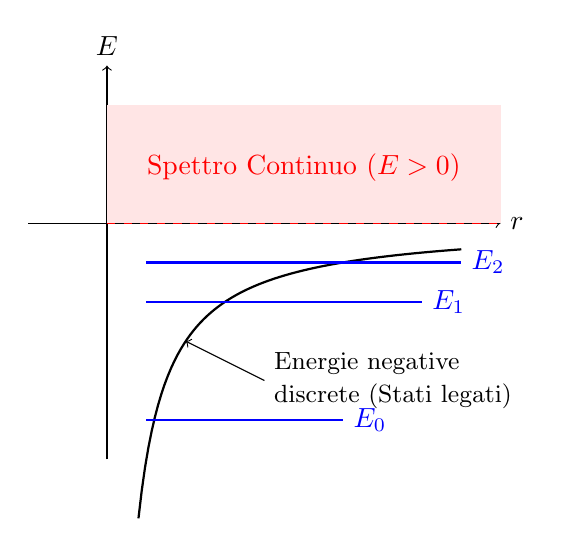
\begin{tikzpicture}
		% Assi
		\draw[->] (-1,0) -- (5,0) node[right] {$r$};
		\draw[->] (0,-3) -- (0,2) node[above] {$E$};
		
		% Potenziale Coulombiano
		\draw[thick, domain=0.4:4.5, samples=100] plot (\x, {-1.5/\x});
		
		% Livelli discreti
		\draw[blue, thick] (0.5, -2.5) -- (3, -2.5) node[right] {$E_0$};
		\draw[blue, thick] (0.5, -1.0) -- (4, -1.0) node[right] {$E_1$};
		\draw[blue, thick] (0.5, -0.5) -- (4.5, -0.5) node[right] {$E_2$};
		
		% Spettro continuo
		\fill[red!10] (0,0) rectangle (5,1.5);
		\draw[red, dashed] (0,0) -- (5,0);
		\node[red] at (2.5, 0.7) {Spettro Continuo ($E > 0$)};
		
		% Annotazioni
		\draw[<-] (1, -1.5) -- (2, -2) node[right, align=left] {\small Energie negative\\ \small discrete (Stati legati)};
	\end{tikzpicture}
\end{center}

Non sappiamo a priori se $\ket{\psi(t)}$ sia uno stato legato o di scattering (o una sovrapposizione). Dobbiamo prendere una base dello spazio $L^2$.
Se dobbiamo trovare le autofunzioni di $H$:
$$
\left[ -\frac{\hbar^2}{2m}\nabla^2 - \frac{e}{4\pi r} \right] \psi = E\psi
$$
Poiché $H$ ha spettro continuo, le soluzioni $\psi$ appartengono allo spazio delle distribuzioni $\Dp$, non necessariamente a $L^2$ (non sono normalizzabili nel senso classico). È un'equazione differenziale su $\Dp$.



\subsection{Indici di difetto e Criteri}

% 
\begin{definizione}[Indici di Difetto]
	Dato un operatore simmetrico $T$, si definiscono indici di difetto le dimensioni dei sottospazi di difetto (nuclei dell'aggiunto shiftato):
	$$ d_{\pm}(T) := \dim[\ker(T^* \mp i\Identity)] $$
\end{definizione}

% - 
\begin{teorema}[Estensioni Autoaggiunte e Indici di Difetto]
	Se $d_+(T) = d_-(T) = k$, allora esistono infinite estensioni autoaggiunte di $T$. Tale famiglia di estensioni è parametrizzata da un gruppo a un parametro $U(\alpha)$ di trasformazioni unitarie (o più in generale da una matrice unitaria $U(k)$).
	Se $d_+(T) \neq d_-(T)$, l'operatore non ammette estensioni autoaggiunte.
	Se $d_+(T) = d_-(T) = 0$, l'operatore è essenzialmente autoaggiunto.
\end{teorema}

% 
\begin{teorema}[Formula di von Neumann per il Dominio]
	Nel caso $d_+(T) = d_-(T) = 1$, siano $\varphi_+ \in \ker(T^*-i\Identity)$ e $\varphi_- \in \ker(T^*+i\Identity)$ vettori normalizzati. Le estensioni autoaggiunte $T_\alpha$ sono in corrispondenza biunivoca con le isometrie suriettive tra i sottospazi di difetto (in questo caso fasi $e^{i\alpha}$). Il dominio dell'estensione $T_\alpha$ è dato da:
	$$ D(T_\alpha) = \{ \psi + z\varphi_+ + z e^{i\alpha}\varphi_- \mid \psi \in D(T), z \in \mathbb{C} \} $$
\end{teorema}

% - - 
\begin{criterio}[Autoaggiunzione essenziale tramite base ortonormale]
	Se un operatore simmetrico $T$ possiede una base ortonormale di autostati $\{\psi_n\}_{n \in \N}$ con autovalori reali, allora $T$ è essenzialmente autoaggiunto, cioè $d_+(T) = d_-(T) = 0$.
\end{criterio}

% 
\begin{criterio}[Coniugazione di von Neumann]
	Sia $\Hspace$ uno spazio di Hilbert e $T: D(T) \to \Hspace$ un operatore simmetrico. Sia $C: \Hspace \to \Hspace$ un operatore antilineare (coniugazione) tale che:
	\begin{enumerate}
		\item $C^2 = \Identity$;
		\item $\innerprod{C\psi}{C\varphi} = \overline{\innerprod{\psi}{\varphi}}$ per ogni $\psi, \varphi \in \Hspace$;
		\item $C(D(T)) \subseteq D(T)$ e $[C, T] = 0$ sul dominio di $T$ (ossia $CT\psi = TC\psi$).
	\end{enumerate}
	Allora gli indici di difetto sono uguali: $d_+(T) = d_-(T)$. Di conseguenza, l'operatore ammette estensioni autoaggiunte.
\end{criterio}

% - 
\begin{osservazione}[Dipendenza dal Dominio Spaziale]
	La natura degli indici di difetto e la possibilità di estensioni autoaggiunte dipendono non solo dall'espressione formale dell'operatore differenziale, ma dalla topologia dell'intervallo su cui è definito.
	Ad esempio, per l'operatore $T = xp + px$:
	\begin{itemize}
		\item Su $\R$: Essenzialmente autoaggiunto ($d_\pm = 0$).
		\item Su un intervallo limitato $(a, b)$ (es. $(1,2)$): Ammette infinite estensioni ($d_\pm = 1$).
		\item Su un intervallo semi-limitato o singolare (es. $(0, 1)$ dove $1/x$ non è integrabile): Può accadere che $d_+ \neq d_-$, rendendo impossibile l'estensione autoaggiunta.
	\end{itemize}
\end{osservazione}

\begin{esempio}[Hamiltoniano dell'Oscillatore Armonico e Autoaggiunzione Essenziale]
	Si consideri l'operatore $H := -\frac{d^2}{dx^2} + x^2$ definito su $\Schwartz(\R)$. Per determinare se è essenzialmente autoaggiunto (senza calcolare esplicitamente gli indici di difetto $d_\pm(H)=0$), utilizziamo il Criterio di Nelson.
	
	\begin{teorema}[Criterio di Nelson]
		Sia $A$ un operatore simmetrico su uno spazio di Hilbert $\Hspace$. Se il dominio di $A$, $D(A)$, contiene un insieme di vettori analitici per $A$ il cui span è denso in $\Hspace$, allora $A$ è essenzialmente autoaggiunto.
	\end{teorema}
	
	\begin{definizione}[Vettore Analitico]
		Un vettore $f \in \Hspace$ è detto analitico per $A$ se esiste $s > 0$ tale che:
		$$ \sum_{n=0}^{\infty} \frac{\|A^n f\| s^n}{n!} < \infty $$
	\end{definizione}
	
	In particolare, gli autovettori propri di $A$ sono vettori analitici (la serie diventa una serie esponenziale convergente).
	Per applicare il criterio, è sufficiente provare che gli autostati dell'oscillatore armonico $\{\psi_n\}_{n \in \N}$ formano un sistema ortonormale completo (s.o.n.c.) per $L^2(\R)$.
	Ricordiamo la forma esplicita:
	$$ \psi_n(x) := \frac{1}{\sqrt{2^n n!}} \left(\frac{1}{\pi}\right)^{1/4} e^{-x^2/2} H_n(x) $$
	dove $H_n(x) = (-1)^n e^{x^2} \frac{d^n}{dx^n}(e^{-x^2})$ sono i polinomi di Hermite.
\end{esempio}

% - 
\begin{esempio}[Dimostrazione: 1. Ortogonalità]
	Per $m \neq n$ (assumiamo $n > m$), dobbiamo mostrare $(\psi_n, \psi_m)_{L^2(\R)} = 0$.
	Questo equivale a mostrare l'ortogonalità dei polinomi di Hermite rispetto al peso $e^{-x^2}$:
	$$ \int_{\R} H_n(x) H_m(x) e^{-x^2} dx = (-1)^n \int_{\R} H_m(x) \frac{d^n}{dx^n}(e^{-x^2}) dx $$
	Integrando per parti $n$ volte (i termini di bordo si annullano per la rapida decrescenza della gaussiana):
	$$ = (-1)^{2n} \int_{\R} e^{-x^2} \frac{d^n}{dx^n}(H_m(x)) dx = 0 $$
	L'ultima uguaglianza vale perché $H_m(x)$ è un polinomio di grado $m < n$, quindi la sua derivata $n$-esima è nulla.
\end{esempio}

% - 
\begin{esempio}[Dimostrazione: 2. Normalizzazione]
	Verifichiamo $\|\psi_n\|^2 = 1$. Ponendo $m=n$ nella formula precedente:
	$$ \|\psi_n\|^2 \propto \int_{\R} \frac{d^n}{dx^n}(H_n(x)) e^{-x^2} dx $$
	Poiché $H_n(x)$ è di grado $n$, la derivata $n$-esima è una costante ($2^n n!$). Portandola fuori dall'integrale rimane l'integrale gaussiano $\int e^{-x^2} dx = \sqrt{\pi}$.
	Combinando i fattori di normalizzazione:
	$$ \|\psi_n\|^2 = \frac{1}{2^n n! \sqrt{\pi}} (2^n n!) \sqrt{\pi} = 1 $$
\end{esempio}

% - 
\begin{esempio}[Dimostrazione: 3. Completezza]
	Dobbiamo mostrare che se $f \in L^2(\R)$ è ortogonale a tutti i $\psi_n$, allora $f=0$.
	Lo span dei polinomi di Hermite coincide con lo span di tutti i polinomi.
	Dobbiamo verificare che $S := \text{span}\{ e^{-x^2/2} p(x) \mid p(x) \text{ polinomio} \}^\perp = \{0\}$.
	Sia $f \in S$. Allora $\int_{\R} f(x) e^{-x^2/2} x^n dx = 0$ per ogni $n$.
	Definiamo $g(x) := f(x) e^{-x^2/2}$. Calcoliamo la trasformata di Fourier di $g$:
	$$ G(\xi) = \int_{\R} f(x) e^{-x^2/2} e^{i\xi x} dx = \sum_{n=0}^{\infty} \frac{(i\xi)^n}{n!} \int_{\R} f(x) e^{-x^2/2} x^n dx = 0 $$
	Poiché $G(\xi) = 0$, per il teorema di Plancherel $\|g\|_{L^2} = \frac{1}{2\pi} \|G\|_{L^2} = 0$, quindi $g(x)=0 \implies f(x)=0$.
	Concludiamo che $H$ è essenzialmente autoaggiunto.
\end{esempio}

% - 
\begin{esempio}[Interpretazione Fisica: Operatore Cinetico su Semiretta]
	Abbiamo visto che $T = -\frac{d^2}{dx^2}$ su $L^2(0, \infty)$ ammette estensioni autoaggiunte $T_\alpha$ definite da condizioni al contorno di Robin:
	$$ f'(0) + \beta f(0) = 0, \quad \beta = \frac{1}{\sqrt{2}}\left(1 + \tan\frac{\alpha}{2}\right) $$
	Possiamo riscrivere la condizione usando un parametro $\gamma \in [-\pi/2, \pi/2]$ tale che $\beta = \tan \gamma$:
	$$ \cos\gamma f'(0) + \sin\gamma f(0) = 0 $$
	\begin{itemize}
		\item $\gamma = 0 \implies f'(0)=0$ (Neumann).
		\item $\gamma = \pm \pi/2 \implies f(0)=0$ (Dirichlet).
	\end{itemize}
\end{esempio}

\begin{osservazione}[Condizioni di Robin e "Skin Effect" (Stati di Bordo)]
	Una conseguenza fisica rilevante delle condizioni al contorno di Robin ($f'(0) + \beta f(0) = 0$) nell'estensione autoaggiunta dell'operatore cinetico è la possibilità di supportare stati localizzati al bordo.
	Come visto precedentemente, per $\beta > 0$ (corrispondente a $\theta \in (0, \pi/2)$ con $\beta = \cot\theta$), l'equazione agli autovalori ammette la soluzione:
	$$ f(x) = C e^{-\beta x} $$
	Questa funzione presenta caratteristiche peculiari:
	\begin{itemize}
		\item \textbf{Localizzazione Esponenziale:} La densità di probabilità $|\psi(x)|^2 \sim e^{-2\beta x}$ è massima al bordo ($x=0$) e decade esponenzialmente verso l'interno del dominio ("bulk"). Questo comportamento è analogo a uno "Skin Effect" quantistico, dove la particella è confinata sulla superficie del materiale.
		\item \textbf{Energia Negativa:} Tale stato corrisponde a un autovalore di energia negativo $E = -\beta^2$. Questo indica uno stato legato creato puramente dalla condizione al contorno, che agisce come una buca di potenziale attrattiva (una "trappola" delta di Dirac al bordo).
		\item \textbf{Dipendenza dal Parametro:} Maggiore è $\beta$, più rapido è il decadimento (minore lunghezza di penetrazione $\lambda \sim 1/\beta$) e più forte è il confinamento al bordo. Se $\beta \to 0$ (condizione di Neumann), lo stato legato scompare e ci si riconduce allo spettro continuo puro.
	\end{itemize}
	In sintesi, le condizioni di Robin permettono di modellizzare interazioni superficiali che possono "catturare" la particella, generando stati che non esistono per le condizioni "pure" di Dirichlet o Neumann.
\end{osservazione}

% - 
\begin{osservazione}[Stati Legati e Problema della Radice Quadrata]
	Consideriamo la funzione $f_\theta(x) = e^{-\cot\theta x}$ con $\theta \in (0, \pi/2)$ (quindi $\cot\theta > 0$).
	Questa funzione è in $L^2(0, \infty)$ e soddisfa la condizione al contorno per $\beta = \cot\theta$.
	$$ T_\alpha f_\theta = -\frac{d^2}{dx^2} (e^{-\cot\theta x}) = -(\cot^2\theta) f_\theta $$
	$f_\theta$ è un'autofunzione con autovalore negativo ($-\cot^2\theta$). Questi sono detti \textbf{stati legati}.
	Ciò implica che l'estensione $T_\alpha$ non preserva la positività dell'operatore originale $T$.
	\textbf{Conseguenza fisica:} Se interpretiamo $T$ come l'energia cinetica $P^2$, non possiamo definire univocamente l'operatore impulso $P = \sqrt{T_\alpha}$ perché lo spettro contiene valori negativi (la radice sarebbe immaginaria).
	Questo riflette il fatto che l'operatore impulso $P = -i\frac{d}{dx}$ su $(0, \infty)$ ha indici di difetto diversi ($d_+=0, d_-=1$) e non ammette estensioni autoaggiunte.
\end{osservazione}

% - 
\begin{esempio}[Operatore Cinetico su Intervallo Limitato]
	Per $T = -\frac{d^2}{dx^2}$ su un intervallo limitato $(a,b)$, gli indici di difetto sono $d_\pm(T) = 2$.
	Le estensioni autoaggiunte sono parametrizzate da una matrice unitaria $U \in U(2)$ (dimensione 4).
	La parametrizzazione può essere scritta come:
	$$ U = e^{i\theta} M, \quad \text{con } M \in SU(2), \theta \in [0, \pi] $$
	$$ M = m_0 \Identity - i \vec{m} \cdot \vec{\sigma} $$
	dove $\vec{\sigma}$ sono le matrici di Pauli e $m_0^2 + |\vec{m}|^2 = 1$.
	Anche in questo caso, le estensioni non garantiscono necessariamente la positività.
\end{esempio}

\subsection{Varie su distribuzioni}

\begin{esempio}[Supporto di $\delta$]
	
	Consideriamo la delta di Dirac $\delta$.
	Se prendiamo una funzione test $\varphi$ supportata su $(x-a, x+b)$ tale che $0 \notin (x-a, x+b)$, allora:
	$$
	\delta(\varphi) = 0
	$$
	Quindi su tutti questi insiemi che non contengono l'origine, la $\delta$ è nulla.
	
	Tuttavia, per ogni $\varepsilon > 0$, definendo un intorno $I_\varepsilon = (-\varepsilon, \varepsilon)$, per ogni $\varphi \in \mathcal{D}(\R)$ con $\text{supp}(\varphi) \subset I_\varepsilon$, abbiamo:
	$$
	\delta(\varphi) = \varphi(0)
	$$
	che può essere diverso da zero. Quindi il supporto è topologicamente l'insieme $\{0\}$.
	Per la funzione gradino di Heaviside $\Theta(x)$ (indicata come $\mathbb{H}$ o $\Theta$ negli appunti), si può dimostrare che:
	$$
	\text{supp}(\Theta) = [0, \infty)
	$$
\end{esempio}

\subsection{Esempi di equazioni distribuzionali}

\begin{esempio}[Pettine di Dirac]
	Risolvere $\sin(x) \cdot u = 0$ con $u \in \Dp(\R)$.
	La soluzione è il cosiddetto \textbf{Pettine di Dirac}:
	$$
	u = \sum_{k \in \mathbb{Z}} c_k \delta_{x_k} \quad \text{con } x_k = k\pi
	$$
\end{esempio}

\begin{esempio}[Cristallo unidimensionale]
	Consideriamo un modello di cristallo descritto dall'Hamiltoniana:
	$$
	H = -\frac{\hbar^2}{2m}\frac{d^2}{dx^2} + \sum_{k \in \mathbb{Z}} \lambda \delta_k
	$$
	Qui vediamo ogni atomo come una delta di Dirac.
	\textbf{Nota:} Questo operatore $H$ \textit{non} può agire rigorosamente su $L^2(\R)$ perché la $\delta$ non è definita su funzioni di $L^2$ (necessita continuità, mentre funzioni $L^2$ sono classi di equivalenza).
\end{esempio}

\subsection{La distribuzione $\frac{1}{x}$}

Vogliamo risolvere l'equazione distribuzionale:
$$
x u = 1 \quad \text{con } u \in \Dp(\R)
$$
Questa è un'equazione non omogenea. La soluzione generale è data dalla somma di una soluzione particolare $u_p$ e della soluzione dell'omogenea $u_0$:
$$
u = u_p + u_0
$$

\subsubsection{Soluzione Omogenea}
L'equazione omogenea è $x u_0 = 0$.
La soluzione è proporzionale alla delta di Dirac (che è supportata in 0, dove $x=0$):
$$
u_0 = c \delta
$$
(Definizione di soluzione particolare e omogenea).

\subsubsection{Soluzione Particolare}
Intuitivamente verrebbe da dire $u_p = \frac{1}{x}$. Tuttavia, la funzione $1/x$ classica non appartiene a $\Dp(\R)$ perché non è localmente integrabile nell'intorno dello zero (la singolarità è troppo forte).
$$
\frac{1}{x} \in \Dp(\R \setminus \{0\}) \implies \text{necessitiamo una regolarizzazione.}
$$
Possiamo usare la derivata del logaritmo:
$$
\frac{1}{x} = \frac{d \ln|x|}{dx}
$$
Sappiamo che $\ln|x| \in L^1_{\text{loc}}$, quindi è integrabile e definisce una distribuzione regolare. Possiamo quindi definire la distribuzione "valore principale di $1/x$" come:
$$
\text{P.V.}\left(\frac{1}{x}\right) := \frac{d}{dx} \ln|x| \in \Dp(\R)
$$

\subsubsection{Verifica Formale}
Per ogni funzione test $f \in \mathcal{D}(\R)$:
$$
\left\langle \frac{d \ln|x|}{dx}, f \right\rangle = - \left\langle \ln|x|, \frac{df}{dx} \right\rangle = - \int_{-\infty}^{+\infty} dx \ln|x| \frac{df}{dx}
$$
Calcoliamo questo integrale separando la singolarità con un limite $\varepsilon \to 0^+$:
$$
W(f) = \lim_{\varepsilon \to 0^+} \left[ \int_{-\infty}^{-\varepsilon} dx \frac{f(x)}{x} + \int_{\varepsilon}^{+\infty} dx \frac{f(x)}{x} \right]
$$
Analizziamo il termine con il logaritmo (usando l'integrazione per parti sul termine distribuzionale):
$$
= \lim_{\varepsilon \to 0^+} \left( \left[ \ln|x|f(x) \right]_{-\infty}^{-\varepsilon} + \left[ \ln|x|f(x) \right]_{\varepsilon}^{+\infty} - \int_{|x|>\varepsilon} dx \ln|x| \frac{df}{dx} \right)
$$
Consideriamo i termini di bordo a $\varepsilon$:
$$
\left[ \ln|x|f(x) \right]_{-\infty}^{-\varepsilon} + \left[ \ln|x|f(x) \right]_{\varepsilon}^{+\infty} = \ln|-\varepsilon|f(-\varepsilon) - \ln|\varepsilon|f(\varepsilon)
$$
Espandiamo $f$ in serie di Taylor attorno a 0: $f(\pm \varepsilon) = f(0) \pm f'(0)\varepsilon + O(\varepsilon^2)$.
$$
= \ln \varepsilon [ f(0) - f'(0)\varepsilon ] - \ln \varepsilon [ f(0) + f'(0)\varepsilon ] + \dots
$$
$$
= \ln \varepsilon [ f(-\varepsilon) - f(\varepsilon) ] = \ln \varepsilon [ (f(0) - f'(0)\varepsilon) - (f(0) + f'(0)\varepsilon) ]
$$
$$
= \ln \varepsilon [ -2\varepsilon f'(0) ] \to 0 \quad \text{per } \varepsilon \to 0
$$
Il primo termine si annulla (o meglio, i termini divergenti si cancellano grazie alla simmetria del Valor Principale).
Quindi:
$$
W(f) = \lim_{\varepsilon \to 0^+} \left( \int_{\varepsilon}^{\infty} dx \frac{f(x) - f(-x)}{x} \right) = \text{P.V.} \int_\R \frac{f(x)}{x} dx
$$
Dunque la distribuzione è ben definita:
$$
\left\langle \frac{d \ln|x|}{dx}, f \right\rangle = \text{P.V.} \left\langle \frac{1}{x}, f \right\rangle
$$

\subsubsection{Soluzione Generale}
La soluzione dell'equazione $x u = 1$ in $\Dp(\R)$ è quindi:
$$
u = \text{P.V.}\left(\frac{1}{x}\right) + c \delta
$$

\subsubsection{Analisi Complessa e Regolarizzazione}

Possiamo vedere la regolarizzazione attraverso l'integrazione nel piano complesso:
$$
\int \frac{f(x)}{x} dx \longrightarrow \oint \frac{f(z)}{z} dz
$$
Consideriamo un percorso che evita la singolarità in $z=0$ deformando il cammino nel piano complesso.
\subsubsection{Calcolo dei residui sui semicerchi}

\begin{enumerate}
	\item \textbf{Percorso $C_\varepsilon$ (sopra il polo):}
	$$
	\lim_{\varepsilon \to 0^+} \int_{C_\varepsilon} \frac{f(z)}{z} dz = i \pi f(0)
	$$
	(Nota: Il segno dipende dall'orientazione. Per il Lemma di Jordan sul piccolo cerchio in senso orario sarebbe $-i\pi \text{Res}$, qui stiamo integrando solo sul semicerchio). Negli appunti è indicato $\pi i f(0)$.
	
	\item \textbf{Percorso $D_\varepsilon$ (sotto il polo):}
	$$
	\lim_{\varepsilon \to 0^+} \int_{D_\varepsilon} \frac{f(z)}{z} dz = - i \pi f(0)
	$$
\end{enumerate}

Questo concetto si lega alle formule di Plemelj-Sokhotski. Spostare il polo $z \to z \pm i\varepsilon$ equivale a deformare il contorno:
$$
\lim_{\varepsilon \to 0^+} \frac{1}{x \mp i\varepsilon} = \text{P.V.}\frac{1}{x} \pm i\pi \delta(x)
$$
Negli appunti troviamo la relazione:
$$
\lim_{\varepsilon \to 0^+} \oint_{C} \frac{f(z)}{z - i\varepsilon} = 2\pi i f(i\varepsilon) \to 2\pi i f(0)
$$

\textbf{Domanda:} Quale di questi risultati è quello giusto per $u$?
\textbf{Risposta:} Tutti. La soluzione generale è $u = \text{P.V.}\frac{1}{x} + c\delta$.
A seconda della fisica del problema (condizioni al contorno, causalità, ecc.), il valore della costante $c$ cambia.

\begin{esempio}[Controesempio finale]
	La funzione $e^{1/x}$ \textbf{non} è interpretabile come distribuzione. La singolarità essenziale in $x=0$ è troppo forte per essere regolarizzata nello spazio delle distribuzioni standard.
\end{esempio}

\subsection{Prodotto tensore}

Voglio descrivere contemporaneamente due sistemi isolati con due spazi di Hilbert, $\Hspace_1$ e $\Hspace_2$.
Prendiamo due operatori $\hat{A}$ su $\Hspace_1$ e $\hat{B}$ su $\Hspace_2$.
Dato che $\psi \in \Hspace_1$ e $\phi \in \Hspace_2$, l'intuizione iniziale potrebbe suggerire che lo spazio totale sia la somma diretta:
\[
\Hspace = \Hspace_1 \oplus \Hspace_2
\]
Quindi considero le coppie $(\psi, \phi) \in \Hspace_1 \oplus \Hspace_2$. La somma diretta è molto naturale (analogamente a $\R^2 = \R + \R$). Come si sommano questi vettori? Componente per componente: $(x+x', y+y')$. Questa è la \textbf{somma diretta} tra due elementi di $\R \times \R$.

Voglio costruire un osservabile che misuri sia $\hat{A}$ che $\hat{B}$. Definiamo:
\[
\hat{A} \oplus \hat{B} : \Hspace_1 \oplus \Hspace_2 \longrightarrow \Hspace_1 \oplus \Hspace_2
\]
Agisce come:
\[
(\psi, \phi) \longmapsto (\hat{A}\psi, \hat{B}\phi)
\]
Questa mappa è lineare? Sì, lo si vede velocemente.

\begin{osservazione}[Il problema dell'interazione]
	Ho fatto l'assunzione che i due sistemi siano \textbf{isolati} (cioè non si "parlano"). Stai anche assumendo che dati $S_1$ e $S_2$, esista un sistema più grande $S$ che li contiene.
	Consideriamo sistemi con interazione, per esempio \textbf{spin-orbita}. L'operatore è $\hat{L} \cdot \hat{S}$, dove $\hat{L}$ è la parte spaziale e $\hat{S}$ è la parte di spin.
	\[
	\hat{L} \cdot \hat{S} : L^2(\R^3) \oplus \C^{2s+1} \longrightarrow L^2(\R^3) \oplus \C^{2s+1} \quad \text{(Ipotesi)}
	\]
	$\hat{L}$ e $\hat{S}$ sono buone osservabili, ma il loro prodotto deve agire congiuntamente. Se usassimo la somma diretta, sorgerebbe un problema di linearità nel combinare gli stati.
\end{osservazione}

\begin{esempio}[Controesempio sulla linearità]
	Prendiamo lo spazio di Hilbert $\R$. Definiamo una mappa $k: \R \oplus \R \longrightarrow \R \oplus \R$ come:
	\[
	(a, b) \longmapsto (ab, 0)
	\]
	Questa mappa è lineare? \textbf{NO}.
	Verifichiamo la linearità sulla somma:
	\[
	k((a,b) + (c,d)) = k(a+c, b+d) = ((a+c)(b+d), 0)
	\]
	Mentre la somma delle immagini sarebbe:
	\[
	k(a,b) + k(c,d) = (ab, 0) + (cd, 0) = (ab + cd, 0)
	\]
	Chiaramente:
	\[
	(a+c)(b+d) = ab + ad + cb + cd \neq ab + cd
	\]
	Quindi la mappa è multilineare ma \textbf{non è lineare}.
\end{esempio}

Però $k$ è lineare nei due sottosistemi! Cioè è \textbf{bilineare}:
\[
k(v_1 + v_2, w) = ((v_1+v_2)w, 0) = (v_1 w + v_2 w, 0) = k(v_1, w) + k(v_2, w)
\]
Questo è un grande problema! Io voglio un operatore \textbf{lineare}. Qui entra in gioco il prodotto tensore.

Vogliamo linearizzare le mappe multilineari.
\begin{teorema}[Proprietà Universale del Prodotto Tensore]
	Esiste ed è unico (a meno di isomorfismi) uno spazio $\Hspace_1 \otimes \Hspace_2$ e una mappa bilineare $\otimes: \Hspace_1 \times \Hspace_2 \to \Hspace_1 \otimes \Hspace_2$ tale che per ogni spazio $W$ e per ogni mappa multilineare $F: \Hspace_1 \times \Hspace_2 \to W$, esiste un'unica mappa lineare $f: \Hspace_1 \otimes \Hspace_2 \to W$ che rende commutativo il seguente diagramma:
	
	\begin{center}
		\begin{tikzcd}[row sep=large, column sep=large]
			\Hspace_1 \times \Hspace_2 \arrow[r, "\otimes"] \arrow[d, "F \text{ (multilin.)}"'] & \Hspace_1 \otimes \Hspace_2 \arrow[dl, "\exists! f \text{ (lineare)}"] \\
			W &
		\end{tikzcd}
	\end{center}
	La relazione è data da:
	\[
	F(\psi, \phi) = f(\psi \otimes \phi)
	\]
\end{teorema}

Quindi, se $f$ è lineare $\implies$ è una buona osservabile. Il postulato della Meccanica Quantistica (MQ) suggerisce che vogliamo trattare anche le interazioni $F$ come osservabili. Grazie al teorema di universalità, questo ci porta necessariamente ad usare $\otimes$.


\subsubsection{Prodotto Tensore di Distribuzioni}
Siano $\phi(x) \in C^\infty(\R^n)$ e $\psi(t) \in C^\infty(\R^m)$.
Siano $u, v \in \mathcal{D}'(\R^n)$. Cos'è $u \otimes v$?

Definiamo il prodotto tensore di funzioni test:
\[
(\phi \otimes \psi)(x, y) = \phi(x)\psi(y) \in C^\infty(\R^{n+m})
\]
Se consideriamo le distribuzioni associate $V_{\phi\psi} \in \mathcal{D}'(\R^{n+m})$, definite come:
\[
V_{\phi\psi}(f) = \int_{\R^{n+m}} dx \, dy \, \phi(x) \psi(y) f(x, y) \quad \forall f \in \mathcal{D}(\R^{n+m})
\]
Possiamo vedere che agisce come il prodotto delle distribuzioni singole. Se $f(x,y) = h(x)g(y)$, allora:
\[
V_{\phi\psi}(h \otimes g) = \int dx \, dy \, \phi(x)\psi(y)h(x)g(y) = U_\phi(h) Z_\psi(g)
\]
dove $U_\phi$ e $Z_\psi$ sono le distribuzioni associate rispettivamente a $\phi$ e $\psi$.

\subsection{Convoluzione}

In Meccanica Quantistica, per una particella a spin $1/2$, la funzione d'onda appartiene a $\psi \in L^2(\R^3) \otimes \C^{2s+1}$.
Possiamo mostrare che:
\[
L^2(\R^3) \otimes \C^{2s+1} \simeq L^2(\R^3, \C^{2s+1})
\]
Questo ci dice fisicamente che possiamo associare ad ogni punto dello spazio i gradi di libertà interni del sistema (spin). Ho un \textbf{campo}.

\begin{definizione}[Convoluzione tra funzioni]
	Date $\phi, \psi$ funzioni (purché l'integrale sia ben definito):
	\[
	(\phi * \psi)(x) := \int_{\R^n} dy \, \phi(y) \psi(x-y)
	\]
\end{definizione}

\begin{esempio}[Esempio: Ricostruzione di immagini]
	Vogliamo generare un'immagine su uno schermo (griglia di pixel). L'interpolazione lineare tra punti discreti crea contorni frastagliati.
	La convoluzione è lo strumento che ci dice come passare da una funzione "a tratti" (continua ma non liscia, o discreta) a una funzione liscia ($C^\infty$) con un errore controllato.
\end{esempio}

\begin{esempio}[Convoluzione di Distribuzioni]
Poniamoci nel caso in cui $\phi * \psi \in C^\infty(\R^n)$. Per ogni $f \in \mathcal{D}(\R^n)$ (funzione test):
\[
U_{\phi * \psi}(f) = \int_{\R^n} dx \left( \int_{\R^n} dy \, \phi(y) \psi(x-y) \right) f(x)
\]
Ponendo $z = x-y \implies x = y+z$:
\[
= \int_{\R^{n} \times \R^n} dz \, dy \, \phi(y) \psi(z) f(y+z) = \langle \phi \otimes \psi, f(y+z) \rangle
\]
Vorremmo estendere questa definizione a $u, v \in \mathcal{D}'(\R^n)$.
\[
\langle u * v, f \rangle := \langle u \otimes v, f(x+y) \rangle \quad \forall f \in \mathcal{D}(\R^n)
\]
\end{esempio}
\begin{osservazione}[Il problema del Supporto]
	C'è un problema: se $f \in \mathcal{D}(\R^n)$ ha supporto compatto, la funzione $F(x,y) = f(x+y)$ definita su $\R^{2n}$ \textbf{non ha supporto compatto}!
	
		
	\begin{center}
		\begin{tikzpicture}[scale=0.8]
			% Assi e griglia di sfondo (opzionale per chiarezza)
			\draw[->] (-4,0) -- (4,0) node[right] {$x$};
			\draw[->] (0,-4) -- (0,4) node[above] {$y$};
			
			% Definizione della striscia corretta (Pendenza -1)
			% Le rette sono del tipo y = -x + c
			% Esempio visuale: striscia tra x+y=-1 e x+y=1
			
			% Coordinate calcolate per stare nel box visibile:
			% Linea superiore (x+y=c2): passa per (-2,3) e (3,-2)
			% Linea inferiore (x+y=c1): passa per (-3,2) e (2,-3)
			
			% Riempimento della striscia
			\fill[pattern=north east lines, pattern color=blue!30] 
			(-3, 2) -- (-2, 3) -- (3, -2) -- (2, -3) -- cycle;
			
			% Disegno delle rette di bordo
			\draw[thick, blue] (-3, 2) -- (2, -3) node[below right] {$x+y=c_1$};
			\draw[thick, blue] (-2, 3) -- (3, -2) node[below right] {$x+y=c_2$};
			
			% Etichetta
			\node[fill=white, inner sep=1pt] at (1.5, 1.5) {$\text{supp}(f(x+y))$};
			
			% Frecce per indicare la direzione costante (opzionale ma utile didatticamente)
			\draw[->, dashed, red] (0,0) -- (-1.5, 1.5) node[midway, left] {\tiny Costante};
		\end{tikzpicture}
	\end{center}
	
	Se $f$ ha supporto in $[-1, 1]$, allora $f(x+y)$ è non nulla nella striscia infinita definita da $-1 \le x+y \le 1$. In un sistema di riferimento ruotato $(x+y, x-y)$, la funzione è a supporto compatto in una variabile ma costante (e quindi illimitata) nell'altra. Poiché $u \otimes v$ è definita su funzioni test a supporto compatto in $\R^{2n}$, la definizione sopra richiede cautela (una delle due distribuzioni deve essere a supporto compatto, $u \in \mathcal{E}'$).
\end{osservazione}

\begin{esempio}[Regolarizzazione]
Possiamo usare la convoluzione per regolarizzare una distribuzione $u$. Sia $\rho \in C_0^\infty(\R^n)$ tale che $\int \rho = 1$ (mollificatore).
Costruiamo una successione $\rho_j(x) = j^n \rho(jx)$ che tende alla $\delta$ di Dirac.
\[
\lim_{j \to \infty} u * \rho_j = u * \delta = u
\]
Ad ogni step, $u * \rho_j$ è una \textbf{funzione liscia} ($C^\infty$). Abbiamo libertà nella scelta di $\rho$ in base a quale informazione fisica vogliamo preservare o "perdere" (recuperandola solo al limite).
\end{esempio}


\subsection{L'operatore derivazione nel problema "Particle in a box"}
Si consideri l'operatore differenziale del primo ordine (associato all'operatore momento quantistico $P = -i \frac{d}{dx}$) su un intervallo limitato $I = [0, 1]$:
\[
A = i \frac{d}{dx}.
\]
Vogliamo analizzare le sue proprietà di autoaggiunzione nello spazio di Hilbert $\Hspace = L^2([0,1])$. 
È noto che l'operatore definito sul dominio minimale (funzioni lisce a supporto compatto, o che si annullano con le derivate ai bordi) è simmetrico ma non autoaggiunto.
La questione centrale che affrontiamo è: \textbf{perché non esiste un'estensione autoaggiunta il cui dominio sia esattamente quello delle funzioni che si annullano agli estremi (condizione di Dirichlet)?}

Ovvero, perché non possiamo scegliere come dominio:
\[
D_{Dirichlet} = \{ \psi \in AC([0,1]) \mid \psi' \in L^2, \psi(0)=0, \psi(1)=0 \}?
\]

\subsubsection{Analisi tramite la Teoria di Von Neumann}

Per rispondere, utilizziamo la teoria delle estensioni di Von Neumann.
Gli indici di difetto dell'operatore $A$ su $[0,1]$ sono $(1, 1)$. Ciò significa che esiste una famiglia a un parametro di estensioni autoaggiunte, parametrizzata da $\alpha \in [0, 2\pi)$.
Le autofunzioni dei sottospazi di difetto $\mathcal{K}_+ = \ker(A^* - i\Identity)$ e $\mathcal{K}_- = \ker(A^* + i\Identity)$ sono le soluzioni delle equazioni differenziali:
\[
i \psi' = \pm i \psi \implies \psi' = \pm \psi.
\]
Normalizzando opportunamente (come da riferimento standard), le funzioni generatrici sono:
\begin{align*}
	\varphi_+(x) &= c_1 e^x \\
	\varphi_-(x) &= c_2 e^{-x}
\end{align*}
dove $c_1, c_2$ sono costanti di normalizzazione non nulle.
Si osservi un fatto cruciale: \textbf{queste funzioni esponenziali non si annullano mai nell'intervallo $[0,1]$.} In particolare:
\[
\varphi_\pm(0) \neq 0, \quad \varphi_\pm(1) \neq 0.
\]

\subsubsection{Struttura del Dominio Autoaggiunto $D_\alpha$}
Secondo il Teorema di Von Neumann, il dominio di una generica estensione autoaggiunta $A_\alpha$ è dato dalla somma diretta del dominio minimale e di un sottospazio generato da una specifica combinazione lineare delle funzioni di difetto.
Esplicitamente:
\[
D_\alpha = \left\{ \psi(x) = f(x) + z \left( \varphi_+(x) + e^{i\alpha} \varphi_-(x) \right) \;\middle|\; f \in D(A_{min}), z \in \C \right\}.
\]
Qui:
\begin{itemize}
	\item $f(x)$ appartiene alla chiusura del dominio minimale. Per definizione, $f$ soddisfa le condizioni nulle ai bordi: $f(0) = f(1) = 0$.
	\item $z$ è un coefficiente complesso arbitrario che controlla la ``quantità'' di funzione di difetto aggiunta.
	\item $\alpha \in [0, 2\pi)$ è il parametro che distingue le diverse estensioni autoaggiunte.
\end{itemize}

\subsubsection{Dimostrazione dell'Impossibilità di Dirichlet}

Supponiamo per assurdo di voler imporre le condizioni di Dirichlet ($\psi(0)=0$ e $\psi(1)=0$) su tutto il dominio $D_\alpha$. Questo significherebbe trovare un valore fisso di $\alpha$ tale che, per ogni $z \in \C$, la funzione $\psi \in D_\alpha$ si annulli ai bordi.

Valutiamo la generica funzione $\psi \in D_\alpha$ agli estremi $x=0$ e $x=1$. Ricordando che $f(0)=f(1)=0$, otteniamo:
\[
\psi(x) = z \left( \varphi_+(x) + e^{i\alpha} \varphi_-(x) \right).
\]
Affinché $\psi$ appartenga al dominio di Dirichlet per $z \neq 0$ (cioè per non ricadere nel dominio minimale non autoaggiunto), dobbiamo avere:
\begin{equation}
	\label{eq:sys}
	\begin{cases}
		\varphi_+(0) + e^{i\alpha} \varphi_-(0) = 0 \\
		\varphi_+(1) + e^{i\alpha} \varphi_-(1) = 0
	\end{cases}
\end{equation}

Sostituendo le espressioni degli esponenziali (assorbendo le costanti di normalizzazione per chiarezza, tanto non sono nulle):
\begin{enumerate}
	\item In $x=0$: $c_1 e^0 + e^{i\alpha} c_2 e^0 = 0 \implies c_1 + c_2 e^{i\alpha} = 0$.
	\item In $x=1$: $c_1 e^1 + e^{i\alpha} c_2 e^{-1} = 0 \implies c_1 e + c_2 e^{-1} e^{i\alpha} = 0$.
\end{enumerate}

Dalla prima equazione ricaviamo il vincolo su $\alpha$:
\[
e^{i\alpha} = -\frac{c_1}{c_2}.
\]
Sostituendo questo nella seconda equazione:
\[
c_1 e + c_2 e^{-1} \left( -\frac{c_1}{c_2} \right) = 0 \implies c_1 e - c_1 e^{-1} = 0.
\]
Dividendo per $c_1$ (che è diverso da zero):
\[
e - \frac{1}{e} = 0 \implies e^2 = 1.
\]
Questa uguaglianza è palesemente \textbf{falsa} in $\R$.
Abbiamo ottenuto una contraddizione.

\begin{osservazione}[Significato della Contraddizione]
	Il sistema \eqref{eq:sys} è sovradeterminato. Abbiamo una sola ``manopola'' ($\alpha$) per cercare di azzerare la funzione in due punti distinti ($0$ e $1$).
	\begin{itemize}
		\item Possiamo scegliere $\alpha$ per azzerare la funzione in $x=0$.
		\item Oppure possiamo scegliere $\alpha$ per azzerare la funzione in $x=1$.
		\item \textbf{Non possiamo fare entrambe le cose contemporaneamente.}
	\end{itemize}
	L'unica soluzione matematica al sistema è $z=0$. Ma se $z=0$, il dominio collassa a $D(A_{min})$, che è un operatore simmetrico ma \textbf{non autoaggiunto}.
\end{osservazione}

Il motivo profondo per cui non possiamo prendere il dominio ``piccolo'' di Dirichlet è legato alla definizione di operatore aggiunto.
Ricordiamo che $D(A^*)$ è l'insieme delle $\phi$ tali che il termine di bordo nell'integrazione per parti svanisce contro ogni $\psi \in D(A)$.

\[
\langle \phi, A\psi \rangle - \langle A\phi, \psi \rangle = i \left[ \overline{\phi}(1)\psi(1) - \overline{\phi}(0)\psi(0) \right].
\]

\begin{enumerate}
	\item Se scegliamo $D(A) = D_{Dirichlet}$ (cioè $\psi(0)=\psi(1)=0$), il termine di bordo a destra è identicamente nullo per \textbf{qualsiasi} valore di $\phi(0)$ e $\phi(1)$.
	\item Di conseguenza, il dominio dell'aggiunto $D(A^*)$ diventa massimale: non ha alcuna restrizione ai bordi.
	\item Pertanto $D(A) \subsetneq D(A^*)$, rompendo l'autoaggiunzione.
\end{enumerate}

Le estensioni autoaggiunte (date dai vari $\alpha$) sono dei compromessi: allargano $D(A)$ imponendo condizioni del tipo $\psi(1) = e^{i\theta}\psi(0)$ (condizioni quasi-periodiche). In questo modo, si impone un vincolo anche su $\phi$ nell'aggiunto, tale da rendere $D(A) = D(A^*)$.

In sintesi, per l'operatore momento (indici 1,1) \textbf{non ci sono abbastanza gradi di libertà} per forzare la funzione a zero su entrambi i bordi mantenendo la struttura unitaria. Questo è possibile solo per operatori del secondo ordine (come $P^2$, indici 2,2), dove i parametri liberi sono quattro.
